\section{Benchmark details}
\label{sec-evaluation-benchmark-details}
Next, we have a closer look at some of the benchmarks and see how the effectiveness of each optimisation depends on the characteristics of the source code. Table \ref{tbl-evaluation-benchmark-characteristics} shows the size of each benchmark, the distribution of the executed bytecode instructions, and both the maximum and average number of bytes on the VM stack. We can see some important differences between the benchmarks. While the sort benchmarks on the left are almost completely load/store bounded, \mybench{XXTEA}, \mybench{RC5} and \mybench{MD5} are much more computation intensive, spending fewer instructions on loads and stores, and more on math or bitwise operations. The left three benchmarks and the \mybench{outlier detection} benchmark have only a few bytes on the stack, but as the benchmarks contain more complex expressions, the number of values on the stack increases.

Tables \ref{tbl-performance-per-benchmark} and \ref{tbl-codesize-per-benchmark} show the performance and code size overhead for each benchmark, split up per instruction category. First, the overhead using the unoptimised compiler and original unoptimised source code is shown, followed by the effect of the source code optimisations. Then the resulting overhead using optimised source but the original AOT compiler is shown, followed by the effect on the total overhead when the different optimisations are incrementally added to the compiler, and finally the resulting overhead per category after applying all optimisations.

First, looking at the effect of the source code optimisations, the performance for all benchmarks improves, except for \mybench{heat detection} which slows down by a small fraction. One of the optimisations done is to store a computed value or value retrieved from an array in a temporary variable if it is known the value will not change and is needed again later. After the optimisations to the AOT compiler have been added, accessing local variables is much cheaper than accessing an array and \mybench{heat detection}'s optimised source is slightly faster. Using the baseline AOT compiler however, the extra loads and stores added by this optimisation are much more expensive, which in this case just tipped the balance to a small loss. 

The source code optimisations also result in an average reduction of the code size overhead in Table \ref{tbl-codesize-per-benchmark}, but it increases for some benchmarks due to inlining of small methods. This particularly affects \mybench{RC5}, for which 10 method calls were inlined. Again, without the other optimisations, the overhead from this more significant. The difference between the inlined and non-inlined versions with all other optimisations applied is shown in Table \ref{tbl-quantitative-results}.

Looking at the compiler optimisations, the improved peephole optimiser and stack caching both target the push/pop overhead. Stack caching can eliminate almost all, and replaces the need for a peephole optimiser, but it is interesting to compare the two. The improved peephole optimiser does well for the simple benchmarks like sorting, \mybench{binary} search and \mybench{outlier detection}, leaving less overhead to remove for stack caching. The more computation intensive benchmarks contain more complicated expressions, which means there is more distance between a push and a pop, leaving more cases that cannot be handled by the peephole optimiser. For these benchmarks, replacing the peephole optimiser with stack caching yields a big improvement.

The benchmarks on the left spend more time on load/store instructions. This results in higher load/store overhead, and the two optimisations that target this overhead, popped value caching and mark loops, have a big impact. For the computation intensive benchmarks, the load/store overhead is much smaller, but the higher stack size means stack caching is very important for these benchmarks.

The smaller benchmarks highlight certain specific aspects of our approach, while the larger \mybench{CoreMark} benchmark covers a mix of different types of processing. As a result, it is an average case in almost every row in Table \ref{tbl-performance-per-benchmark}.
% The reason it ends up being the third slowest after all optimisations was discussed in \ref{sec-evaluation-coremark-non-automatic-optimisations}. With the non-automatic optimisations described there, \mybench{CoreMark}'s performance overhead would be 59\%, close to the average of the other benchmarks.

\subsubsection{Bubble sort}
\label{sec-evaluation-bubble-sort}
Next we look at \mybench{bubble sort} in some more detail. After optimisation, most of the stack related overhead has been eliminated and of the 101.2\% remaining performance overhead, most is due to other sources. For \mybench{bubble sort} there is a single, clearly identifiable source. The detailed trace output shows that 79.8\% is due to \mycode{ADD} instructions, but \mybench{bubble sort} hardly does any additions. This is a good example of how the simple JVM instruction set leads to less efficient code. To access an array the VM needs to calculate the address of the indexed value, which takes one move and five additions for an array of shorts. This calculation is repeated for each access. The C version is more efficient, using the auto-increment version of the ATmega's LD and ST instructions to slide a pointer over the array. Of the remaining 101.2\% overhead, 93.1\% is caused by these address calculations.
% ADD, ADC and ADIW all cost 26.6\%. Each array access does 1 MOVW, 2 ADDs, 2 ADCs and 1 ADIW.
% 26.6*3+26.6/2 = 93.1

%\paragraph{Bit shifts} Interestingly, the reason \mybench{FFT} is the slowest, is similar to the reason \mybench{RC5} is fastest: they both spend a large amount of time doing bit shifts. \mybench{RC5} shifts by a variable, but large number of bits. Only 8.0\% of the executed bytecode instructions are bit shifts, but they account for 71\% of the execution time in the optimised version. For these variable bit shifts, our translator and \mycode{avr-gcc} generate a similar loop, so the two share a large constant factor.
%
%On the other hand \mybench{FFT} is a hard case because it does many constant shifts by exactly 6 bits. For these, our VM simply emits 6 single shifts, which is slower than the special case \mycode{avr-gcc} emits for shifts by exactly 6 bits.  While we could do the same, we feel this special case is too specific to include in our VM.

\subsubsection{HeatCalib and FFT}
Table \ref{tbl-codesize-per-benchmark} shows that after optimisation the \mybench{HeatCalib} benchmark has a negative code size overhead. This is caused by the fact that the C versions are compiled using \mycode{avr-gcc}'s -O3 optimisations, optimising for performance instead of code size. In this case, as well as for \mybench{FFT}, this caused \mycode{avr-gcc} to duplicate a part of the code, which improves performance but at the cost of a significantly larger code size.

\subsubsection{MoteTrack}
The \mybench{MoteTrack} benchmark is by far the slowest of our benchmarks, at a 156\% overhead compared to native C. \mybench{MoteTrack} stores a database of reference signatures in flash memory. In C this is a complex struct containing a number of sub-structures and fixed-sized arrays. In Java this becomes a collection of objects and arrays, shown in Figure \ref{fig-motetrack-refsignature-objects}.

Since the layout of the complete C structure is known at compile time, the C function to load a reference signature from the database can simply use \mycode{memcpy_P} to copy a block of 80 bytes from flash memory to RAM. In Java, the method to read from flash memory must follow several references to find the locations to put each value. As a result, reading a single signature takes 1455 cycles in Java, and only 735 cycles in C.
% 68.5% overhead from reading refSignatures from flash. 68.5 / 1695 * 735 = 29.7

After the reference signature is loaded, the fixed offsets in the C structure means \emph{using} the loaded signature is also more efficient in C than in Java, which must again follow a number of references to reach the data. We discuss this in more detail in Section \ref{sec-nested-data}.

\subsubsection{LEC}
In Section \ref{sec-introduction-performance} we calculated that the LEC compression algorithm reduced the energy spent to transmit the sample ECG data by 650 μJ, at the expense of 246 μJ spent on CPU cycles compressing the data, when implemented in C and using the ATmega128 CPU and CC2420 radio.

A compression algorithm like LEC is a good example of an optimisation that may be part of an application loaded onto a sensor node. However, if the overhead of using a VM is too high, the cost of compression may outweight the energy saved on transmission. Table \ref{tbl-performance-per-benchmark} shows that using the baseline AOT approach, the \mybench{LEC} benchmark has an overhead of 885.3\%, which drops to 272.6\% after optimising the source code to avoid repeatedly creating a small object. This means the CPU has to stay active longer, and compressing the data would cost $246 \mu J * 3.726 \approx 917 \mu J$, which is more than the 650 μJ saved on transmission.

After we apply our optimisations, the overhead is reduced to 84.6\%, resulting in $246 \mu J * 1.846 \approx 454 \mu J$ spent on compression. While the savings are less than when using native C to compress the data, our optimisations mean that in this scenario, we can save on transmission costs by using LEC compression, while using the baseline AOT approach, LEC compression would have resulted in a net loss.

\subsubsection{XXTEA and the mark loops optimisation}

\begin{figure}
\centering
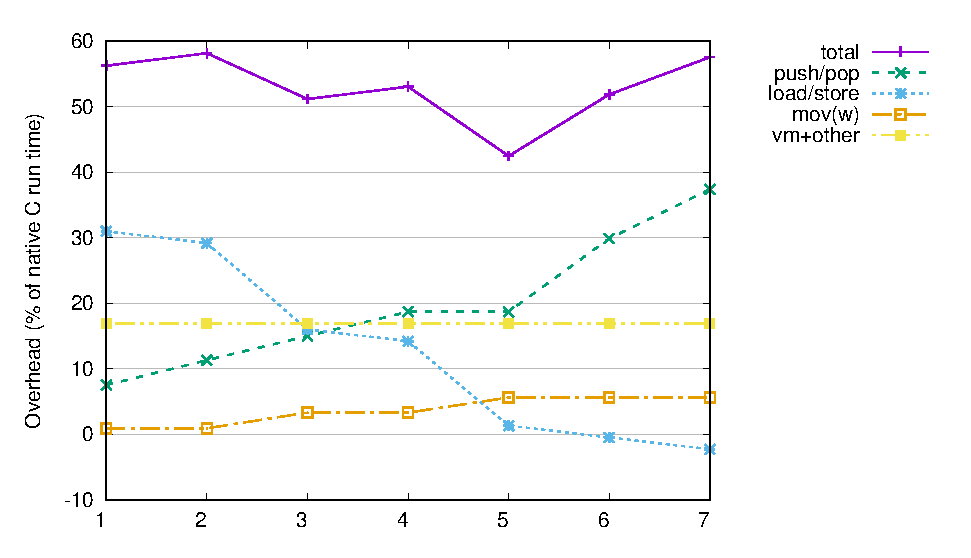
\includegraphics[width=\mygraphsize]{pinnedregs-performance-xxtea.eps}
\caption{XXTEA performance overhead for different number of pinned register pairs}
\label{fig-performance-pinnedregs-xxtea-per-opcode-category}
\end{figure}

\begin{figure}
\centering
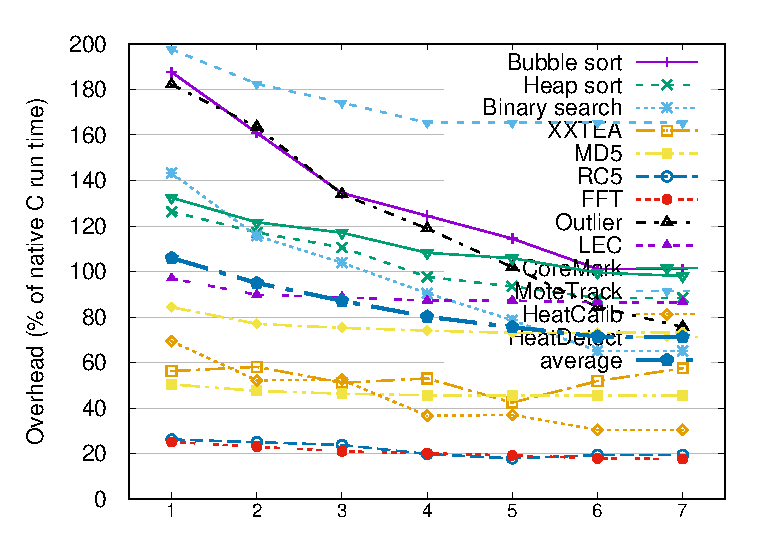
\includegraphics[width=\mygraphsize]{pinnedregs-performance-all-benchmarks.eps}
\caption{Per benchmark performance overhead for different numbers of pinned register pairs}
\label{fig-performance-pinnedregs-per-benchmark}
\end{figure}

The \mybench{XXTEA} benchmark has the highest average stack depth of all benchmarks. As a result, popped value caching does not have much effect: most registers are used for real stack values, leaving few chances to reuse a value that was previously popped from the stack. 

When the mark loops optimisation is applied, performance actually degrades by 5\%! Here we have an interesting trade-off: if a register is used to pin a variable, accessing that variable will be cheaper, but this register will no longer be available for stack caching, so more stack values may have to be spilled to memory.

For most benchmarks, using the maximum of 7 register pairs to pin variables was also the best option. At a lower average stack depth, the fewer number of registers available for stack caching is easily compensated for by cheaper variable access. For \mybench{XXTEA} however, the cost of spilling more stack values to memory outweighs the gains from cheaper variable access when too many variables are pinned. Figure \ref{fig-performance-pinnedregs-xxtea-per-opcode-category} shows the overhead for \mybench{XXTEA} from the different instruction categories. When the number of register pairs used to pin variables is increased from 1 to 7, the load/store overhead steadily decreases, but the push/pop and move overhead increase. For \mybench{XXTEA}, the optimum is at 5 pinned register pairs, at which the total overhead is only 43\%, instead of 58\% at 7 pinned register pairs.

Interestingly, when we pin 7 pairs, the AOT version does fewer loads and stores than the C compiler. Under high register pressure the C version may spill a register value to memory and later load it again, adding extra load/store instructions. When the AOT version pins too many registers, it will also need to spill values, but this adds push/pop instructions instead of loads/stores.

Figure \ref{fig-performance-pinnedregs-per-benchmark} shows the performance for each benchmark, as the number of pinned register pairs is increased. The benchmarks stay stable or even slow down when the number pinned pairs is increased beyond 5 are the benchmarks that have a high stack depth, while the benchmarks with low stack depth such as sort, \mybench{binary search} and \mybench{outlier detection} improve significantly. It should be possible to develop a simple heuristic to allow the VM to make a better decision on the number of registers to pin. Since our current VM always pins 7 pairs, we used this as our end result and leave this heuristic to future work.

